\documentclass{frama-c-book}

\usepackage[T1]{fontenc}
\usepackage[utf8]{inputenc}
\usepackage{tikz}

\usetikzlibrary{fit}
\usetikzlibrary{arrows.meta}
\usetikzlibrary{shapes.geometric}
\usetikzlibrary{positioning}

\usepackage{graphicx}
\usepackage{xspace}
\usepackage{listings}
\usepackage{ifthen}
\usepackage{amsmath,amssymb,amsfonts}
\usepackage{url}
\usepackage{color}
\usepackage{hyperref}
\usepackage{xcolor}
\definecolor{gris}{rgb}{0.95,0.95,0.95}
\definecolor{GrisClair}{rgb}{0.98,0.98,0.98}
\usepackage[leftbars]{changebar}
\usepackage{courier}
% BNF grammar
\newcommand{\indextt}[1]{\index{#1@\protect\keyword{#1}}}
\newcommand{\indexttbs}[1]{\index{#1@\protect\keywordbs{#1}}}
\newif\ifspace
\newif\ifnewentry
\newcommand{\addspace}{\ifspace ~ \spacefalse \fi}
\newcommand{\term}[2]{\addspace\hbox{\lstinline|#1|%
\ifthenelse{\equal{#2}{}}{}{\indexttbase{#2}{#1}}}\spacetrue}
\newcommand{\nonterm}[2]{%
  \ifthenelse{\equal{#2}{}}%
             {\addspace\hbox{\textsl{#1}\ifnewentry\index{grammar entries!\textsl{#1}}\fi}\spacetrue}%
             {\addspace\hbox{\textsl{#1}\footnote{#2}\ifnewentry\index{grammar entries!\textsl{#1}}\fi}\spacetrue}}
\newcommand{\repetstar}{$^*$\spacetrue}
\newcommand{\repetplus}{$^+$\spacetrue}
\newcommand{\repetone}{$^?$\spacetrue}
\newcommand{\lparen}{\addspace(}
\newcommand{\rparen}{)}
\newcommand{\orelse}{\addspace$\mid$\spacetrue}
\newcommand{\sep}{ \\[2mm] \spacefalse\newentrytrue}
\newcommand{\newl}{ \\ & & \spacefalse}
\newcommand{\alt}{ \\ & $\mid$ & \spacefalse}
\newcommand{\is}{ & $::=$ & \newentryfalse}
\newenvironment{syntax}{\begin{tabular}{@{}rrll@{}}\spacefalse\newentrytrue}{\end{tabular}}
\newcommand{\synt}[1]{$\spacefalse#1$}
\newcommand{\emptystring}{$\epsilon$\spacetrue}
\newcommand{\below}{See\; below}

\makeatletter
\newboolean{extension}
\setboolean{extension}{false}

\newenvironment{new}{%
\ifthenelse{\boolean{extension}}%
{\let\full@i\relax\let\endfull@i\relax}%
{\def\full@i{\setbox\z@\vbox\bgroup}%
\def\endfull@i{\egroup}}%
\full@i%
\begin{changebar}\color{red}\bgroup}
{\egroup\end{changebar}\endfull@i}
\makeatother

\newcommand{\machineboxGrisee}[1]{\centerline{%
  \colorbox{GrisClair}{%
    \parbox[t]{4cm}{
  \vspace*{-3ex}
  \begin{tabbing}
%   X\=X\=X\=X\=X\=X\=X\=X\=X\=X\=X\=X\=X\= \kill
  X\=X\=X\=X\=X\=XX\=XX\=XX\=XX\=XX\=XX\=XX\=XX\= \kill
  #1
  \end{tabbing}
  \vspace*{-3ex}
  }}%
   }%
}

\newcommand{\boiteGrise}[2]{\centerline{%
  \colorbox{GrisClair}{
    \parbox[t]{#1}{%
%     \vspace*{-2ex}
    #2
%     \vspace*{-1ex}
  }}%
   }%
}

%%%% Symboles logiques %%%%%%%%%%%%%%%%%%%%%%%%%%%%%%%%%%%%%%%%%%%%%%%%%%

\newcommand{\true}{\mathsf{true}} % true
\newcommand{\false}{\mathsf{false}} % false
\newcommand{\logand}{~\wedge~}    % symbole and
\newcommand{\logor}{~\vee~}   % symbole or
\newcommand{\logimpli}{\Rightarrow} % symbole implique logique
\newcommand{\logequiv}{\Leftrightarrow} % symbole equivalent logique
\newcommand{\bdef}{~\hat =~}    % symbole de d\'efinition

%%%%%%%%% Divers %%%%%%%%%%%%%%%%%%%%%%%%%%%

\newcommand{\bigor}{\mathsf{OR}}  % ou generalise (article FME)
\newcommand{\dirp}[1]{\otimes_{#1}} % produit direct + operation binaire

\newcommand{\biter}{{\sc iterate}}
\newcommand{\bunion}{{\sc union}}
\newcommand{\bUnion}{{\sc UNION}}
\newcommand{\bimpl}{\Rightarrow}

\newcommand{\aorai}{Aora\"i\xspace}
\newcommand{\buchi}{\textnormal{B\"uchi}\xspace}
\newcommand{\ltltoba}{\textit{LTL2BA}}

\newcounter{CptrDefs}
\newcommand{\CorpsDef}{
  \vskip 5pt
    \refstepcounter{CptrDefs}
    \noindent $\!\!\!\!\!\!$ \vrule width 2pt ~ 
    \begin{minipage}{ \textwidth}
      \noindent \textbf{Definition \theCptrDefs ~}
      \itshape
}
\newenvironment{definition}[1]
               {\CorpsDef {\bf (#1)}
                }
               {\end{minipage}
                \mdseries
                \vskip 5pt
               }

\newcommand{\axiom}{\textit{\textbf{axiom}}}
\newcommand{\logic}{\textit{\textbf{logic}}}
\newcommand{\integer}{\textit{\textbf{integer}}}
\newcommand{\axiomatic}{\textit{\textbf{axiomatic}}}
\newcommand{\predicate}{\textit{\textbf{predicate}}}
\newcommand{\transStart}{\textit{transStart}}
\newcommand{\transStop}{\textit{transStop}}
\newcommand{\transCond}{\textit{transCond}}

\newcommand{\curStates}{\lstinline|aorai_CurStates|\xspace}
\newcommand{\curTrans}{\textit{curTr}}
\newcommand{\curStatesOld}{\textit{buch\_CurStates\_old}}
\newcommand{\curStatus}{\textit{Status}}
\newcommand{\curOp}{\textit{Operation}}

\newcommand{\requires}{\textbf{requires}}
\newcommand{\ensures}{\textbf{ensures}}
\newcommand{\assumes}{\textbf{assumes}}
\newcommand{\behavior}{\textbf{behavior}}
\newcommand{\result}{\backslash\textbf{result}}
\newcommand{\old}{\backslash\textbf{old}}


%\setboolean{extension}{true}

\lstdefinelanguage{ya}{
  alsoletter={\\,\%,\$},
  morekeywords={CALL,RETURN,COR,return,true,false,transitions,\\result,other},
  keywordsprefix={\%},
}

\lstloadlanguages{[ANSI]C,[Objective]Caml,csh,ACSL,ya}
\lstset{
basicstyle=\ttfamily,
keywordstyle=\bfseries,
mathescape=false
}

\newcommand{\framacversion}%
           {\input{../../VERSION} (\input{../../VERSION_CODENAME}\unskip)}

\title{\aorai\ Plugin Tutorial\\\textit{\normalsize (A.k.a. LTL to ACSL)}}
\author{Nicolas Stouls and Virgile Prevosto\\
\small\textit{Nicolas.Stouls@insa-lyon.fr},\textit{virgile.prevosto@cea.fr}}

\fcversion{\framacversion}

\cclicence{by-sa}
\copyrightstarts{2009}

\begin{document}
\sloppy
\emergencystretch 3em

\maketitle

\section*{Foreword}
\aorai is a Frama-C plugin that provides a method to automatically annotate a
C program according to an automaton $F$ such that, if the annotations
are verified, we ensure that the program respects $F$. A classical method to
validate annotations then is to use Eva or WP.

This document requires basic knowledge about
the Frama-C platform itself (See \url{https://frama-c.com} for more information),
in particular the notions of {\it plug-ins} and {\it project}.

\vspace*{20pt}
\noindent \textbf{Notes:}
\begin{itemize}
  \item to the question "Why this name: \textit{\aorai}?"
    my answer is: why not? \aorai is the name of the tallest reachable
    mount in the Tahiti island and its reachability is not always obvious.
\end{itemize}

\vspace*{20pt}
\noindent \textbf{Official website:}

\begin{center}
  \url{https://www.frama-c.com/fc-plugins/aorai.html}
\end{center}

\tableofcontents

% ==========================================================================
% ==========================================================================
% ==========================================================================
\chapter{Introduction}
\section{Installation}

\aorai is part of the main Frama-C distribution and is installed by default
with Frama-C. Installation instructions for Frama-C are available at
\url{https://frama-c.com/html/get-frama-c.html}.

\section{Interest of \aorai}

As explained before, \aorai 's goal is to prove that the C program
works like a given automaton. The approach used by \aorai has two
advantages:
\begin{itemize}
\item the high level of abstraction helps to write simple automata and
  avoid the necessity to compute all possibilities of a
  function\footnote{for more information, see
    chapter~\ref{hackers_guide}}
\item thanks to the collaboration between human and plugin principle,
  you can easily check complex C programs (see
  section~\ref{collaboration})
\end{itemize}

\section{Documentation's description}

This document is divided into four parts:
\begin{itemize}
\item First part is a quick overview of \aorai. It will enable you to
  verify basic properties and explain the general principle of the
  software.
\item The second part defines the \aorai input language with which it is
possible to describe a given property.
\item The third part explains how to prove a program annotated with \aorai
using the WP plug-in.
\item Finally, the last part details \aorai's underlying theory, and its
internal architecture in order to help people who would like to contribute to
the plug-in itself.
\end{itemize}

% ========================================================================
% ========================================================================
% ========================================================================
\chapter{Quick overview}

In this chapter we will see how to use Frama-C and the couple
WP-\aorai to prove that a C program has the same behavior as
an automaton.

\section{First use}
\label{first_use}
  The goal is to launch the examples\footnote{ From \url{http://frama-c.com/aorai.html}} and read results.
\subsection{Launching the test}
  First, we will forget about the specification of the automaton,
  which will be described in the second part. In fact, we consider
  that we have already written the file which describes the automaton.

  WP verification\footnote{For more information about WP
    and code verification, please refer to
    \url{http://frama-c.com/wp.html}} can only be done on C
  code augmented with ACSL annotations. Thus,
  \aorai creates a new C file where the automaton is encoded into ACSL
  annotations. Section~\ref{generated_annotated_file} will give more
  information about the annotations generated by \aorai

  If you look at the example's archive, you will find two files:
\begin{itemize}
  \item \texttt{example.ya} which gives a description of the automaton's
    specifications.
  \item \texttt{example.c} is the implementation which will be checked.
\end{itemize}

 With these two files (automaton's description and C file), we can create an
annotated file. This
is done by the following command:
\begin{frama-c-commands}
\$ frama-c example.c -aorai-automata example.ya \
          -then-last -ocode example_annot.c -print
\end{frama-c-commands} %$

This generates a new C file \texttt{example\_annot.c}.
In order to decide if the original program is correct with respect to
the automaton, it is sufficient to establish that the generated C code and
its associated ACSL annotations are valid. For instance, the following command
uses the WP plugin over the generated file:
\begin{frama-c-commands}
\$ frama-c example_annot.c -wp -wp-rte
\end{frama-c-commands} %$

Of course, any option of WP itself can be used, notably \texttt{-wp-rte} to
check for the absence of runtime error.
Finally, it is possible to instruct Frama-C to do a
sequence of analyzes over various projects, {\it via} the \texttt{-then-on}
options and \texttt{-then-last} options.
Thus, we do not need to use an intermediate file and to run Frama-C
twice. Instead, we just instruct WP to operate on the \texttt{aorai}
project that contains the code annotated by \aorai:
\begin{frama-c-commands}
\$ frama-c example.c -aorai-automata example.ya \
          -then-last -wp -wp-rte
\end{frama-c-commands} %$

\subsection{Automata and verification}
The main interest of \aorai is to prove that the program can be
described by an automaton. Please keep in mind that solutions to
write automata in \aorai are listed in the next chapter.

 The automaton of our running example is described by
 figure~\ref{BuchiExample}.

  \begin{figure}[htb]
    \centerline{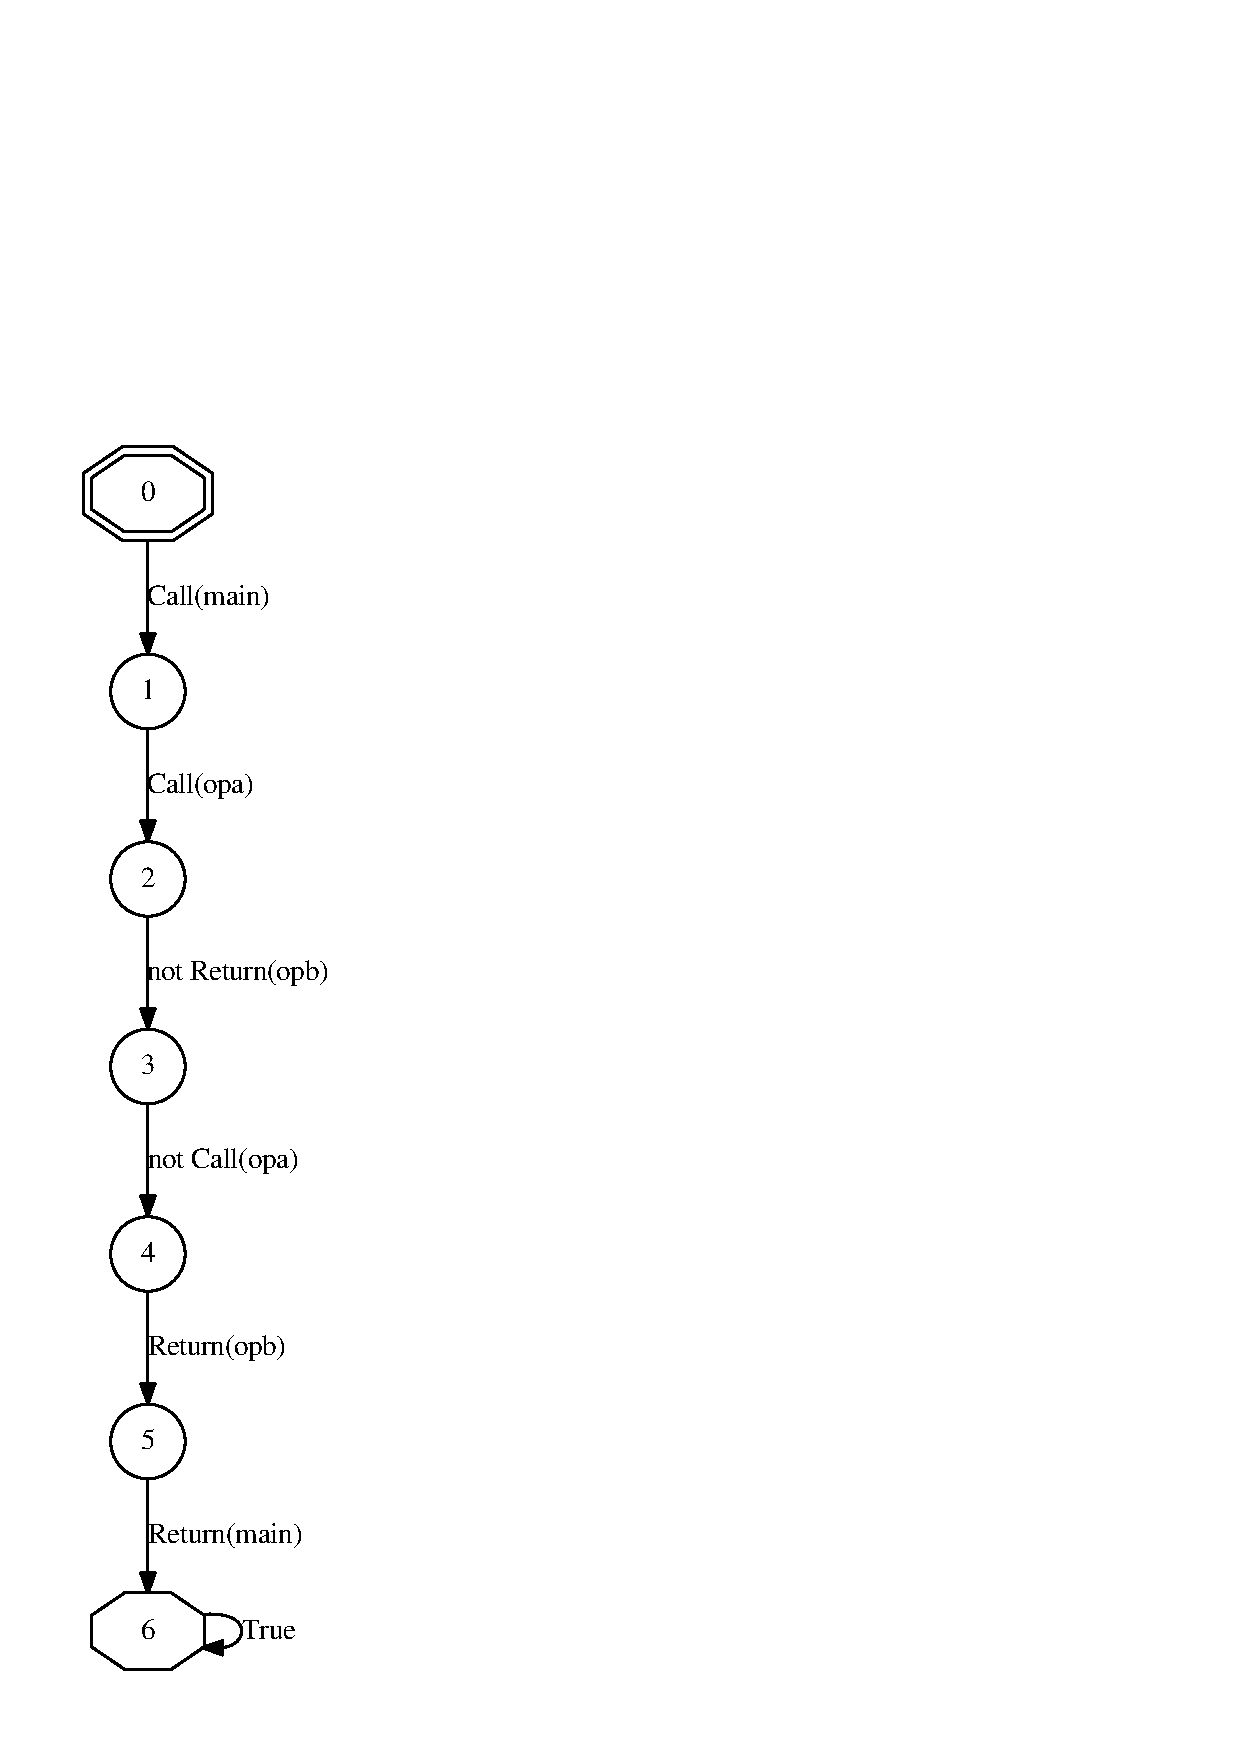
\includegraphics[height=\textheight]{Schemas/example}}
    \caption{Automaton}
    \label{BuchiExample}
  \end{figure}

  From the description contained in {\tt .ya} file, a
  specification --- in
  terms of automata states and transitions --- is
  computed for each operation. For instance, the following specification
  corresponds to the previous automaton: \vspace{10pt}

\centerline{  \begin{tabular}{rl}
    opa & $\left \{ \begin{array}{ll}
             \textnormal{Pre :} & state=\{2\} \logand trans=\{1\}\\
             \textnormal{Post :} & \setminus old(state)=\{2\} \bimpl state=\{3\} \logand trans=\{2\}\\
           \end{array} \right.$\vspace{10pt}\\
    opb & $\left \{ \begin{array}{ll}
             \textnormal{Pre :} & state=\{4\} \logand trans=\{3\}\\
             \textnormal{Post :} & \setminus old(state)=\{4\} \bimpl state=\{5\} \logand trans=\{4\}\\
           \end{array} \right.$\vspace{10pt}\\
    opc & $\left \{ \begin{array}{ll}
             \textnormal{Pre :} & state=\emptyset \logand trans=\emptyset\\
             \textnormal{Post :} & \setminus old(state)=\emptyset \bimpl state=\emptyset \logand trans=\emptyset\\
           \end{array} \right.$\vspace{10pt}\\
    main & $\left \{ \begin{array}{ll}
             \textnormal{Pre :} & state=\{1\} \logand trans=\{0\}\\
             \textnormal{Post :} & \setminus old(state)=\{1\} \bimpl state=\{6\} \logand trans=\{5\}\\
           \end{array} \right.$\vspace{10pt}
  \end{tabular}
}

Finally, the C-code which will be checked is given in
figure~\ref{example_c_file}.

\begin{figure}[htb]
\lstinputlisting[style=c]{example/example.c}
\caption{Example of C File}
\label{example_c_file}
\end{figure}

Actually, the mapping between state and code is made thanks to the
transitions properties like \emph{CALL(opa)}. Note that
the pre- and post-conditions of the C functions are defined by the set
of states authorized just before (resp. after) the call.

\aorai generates a new C program, including the automaton
axiomatization, some coherence invariants, and annotations on
operations, such that if this annotated program can be validated with
the WP plugin, then we ensure that it respects the given
properties.

Sometimes, the automaton has not enough information to check the
validity of the C-program, and the problem is only related to the
implementation which is used. In this case you can add some properties
in the automaton \emph{or} in the generated files. For more
information about that, please read section \ref{collaboration}.

\section{Help Command}\label{sec:help-command}

 The \texttt{frama-c -aorai-help} command returns the list of options for the
 \aorai plug-in. Here are the most common ones:
 \begin{description}
   \item[-aorai-automata <f>] considers the property described by the ya
     automata (in Ya language) from file \texttt{<f>}
   \item[-aorai-verbose <n>] gives some information during computation,
     such as used/produced files and heuristics applied
   \item[-aorai-show-op-spec] displays, at the end of the process, the computed specification of each operation, in terms of states and transitions.
   \item[-aorai-dot] generates a dot file of the automata.
     Dot is a graph format used by the
     GraphViz tools\footnote{\url{http://www.graphviz.org}}.

 \end{description}

\section{Known Restrictions}

The current version of \aorai is under development. Hence, there are
some restrictions.
\begin{itemize}
\item Only safety properties can be checked. The liveness
  part is not truly considered. Namely, the acceptance condition is a post-condition
  of the main function, so that we need a terminating program to actually validate
  it: for a non-terminating program, the point where it is supposed to be checked is
  unreachable.
%   \item Currently, the \texttt{switch} and \texttt{unordered} statements are not supported.
  \item Function pointers are only supported if each indirect call comes with
    an \lstinline|calls| ACSL annotation (see Frama-C user manual for more information)
  \item In the init state from the automaton, conditions on C-array or
    C-structure are not statically evaluated (it's an optimization)
    but are supported.
\end{itemize}


% ============================================================================
% ============================================================================
% ============================================================================
\chapter{\aorai's Language}
\aorai's verification principle is built from the
automaton. Automata can be described in the YA language, which was created for \aorai.

\section{YA}
\label{sec:ya}
\lstset{language=ya}
\subsection{YA file}\label{sec:ya-file}
A YA file follows the grammar described in Fig.~\ref{ya-file}.
\begin{figure}[htb]
\input{ya_file.tex}
\caption{Structure of a YA file}\label{ya-file}
\end{figure}
The directives specify the initial and accepting state(s). There must be at
least one initial state (exactly one if the automaton is supposed to be
deterministic). All initial and accepting state must appear in the list of
states afterwards.

A state is simply described by its name and the list of transitions
starting from this state with their guard. The specific \lstinline|other|
guard indicates that this transition is taken if none of the other ones
can be taken. If it appears, it must be last in the list of transitions.

Conditions that can occur in guards are described in the next section.

\begin{new}
By default, \aorai considers that all functions calls and returns trigger
a transition of the automaton. In order to have transitions only for the
functions that explicitly appear in the description of the automaton, the
following directive must be used:
\begin{lstlisting}[language=ya]
%explicit transitions;
\end{lstlisting}
\end{new}

\subsection{Basic YA guards}\label{sec:basic-ya-guards}
The syntax for basic YA conditions is described in
figure~\ref{fig:basic_ya}.
\lstset{language=ya}
\begin{figure}
\input{basic_ya.tex}
\caption{Basic YA guards}\label{fig:basic_ya}
\end{figure}

Basically, a condition is a logical expression obtained from the following
atoms:
\begin{itemize}
\item \lstinline|CALL|, \lstinline|RETURN| or \lstinline|COR| event, indicating
  respectively the call, the return, the call or the return
  of the corresponding function;
\item A relation over the variables of the programs. In addition to global
variables, that are directly accessed through their \lstinline|id|,
it is possible to consider the value returned by a function or the value of
its formal parameters. This is done through
\lstinline|f().return| and \lstinline|f().a| respectively.
In order to be closer to ACSL's syntax,
\lstinline|f().\result| is accepted as a synonym
of \lstinline|f().return|.
\end{itemize}

Whenever \lstinline|f().prm| appears in a relation, the
related guard has an implicit \lstinline|CALL(f)| event, while
\lstinline|f().return|
and \lstinline|f().\result| trigger a \lstinline|RETURN(f)| event.
Note that this might result in an always-false guard if several such
expressions occur in the same guard, as in
\begin{lstlisting}[language=ya]
f().x <= g().y
\end{lstlisting}
In order for this guard to hold, we should be calling at the same time \verb+f+
and \verb+g+, which is not possible. In addition, if such expression occurs in
a negative occurrence, that is under a negation, as in
\begin{lstlisting}[language=ya]
! f().x <= 4
\end{lstlisting}
the related \lstinline|CALL(f)| event itself is {\it not} negated.
In other words,
the guard above is true if and only if we call \lstinline|f| with an argument
greater than \lstinline|4|. Usage of these expressions might be deprecated in
future versions of \aorai in favor of the less ambiguous constructions
presented in the next subsection.

For instance, the automaton used in the chapter~\ref{first_use} contains the
following transitions:
\begin{lstlisting}[language=ya]
%init: S0;
%accept: S0, S1, S2,S3,S4,S5,S6;
S0 : { CALL(main) }  -> S1;
   ;
S1 : { opa().r<5000 }   -> S2
   ;
S2 : { opa().return<=5000 }  -> S3
   ;
S3 : { !RETURN(opa) } -> S4
   ;
S4 : { RETURN(opb) } -> S5
   ;
S5 : { RETURN(main)} -> S6
   ;
S6 : -> S6
   ;
\end{lstlisting}

\subsection{YA extensions}\label{sec:ya-extensions}
\subsubsection{Extended YA guards}
In order to describe more easily whole sequences of calls, some extensions to
the basic conditions above are available. They are described in
figure~\ref{fig:ya-extensions}. Note however that these extensions are very
experimental yet

\lstset{language=ya}

\begin{figure}[ht]
  \input{extended_ya.tex}
  \caption{Extended YA guards}
  \label{fig:ya-extensions}
\end{figure}

A guard can now be the succession of several atomic events, possibly optional
or on the contrary repeated more than one time. The repetition modifier
follows the syntax and semantics of POSIX regexps: the most general are
\lstinline|{e1,e2}| that indicates at least \lstinline|e1| repetitions and at
most \lstinline|e2| and \lstinline|{e1,}| that indicates at least
\texttt{e1} repetitions without upper bound. There are then shortcuts for the
most common patterns:
\begin{itemize}
\item no modifier indicates exactly one execution (equivalent to
\lstinline|{1,1}|)
\item \lstinline|+| indicates 1 or more repetitions
(equivalent to \lstinline|{1,}|)
\item \lstinline|*| indicates any number of repetitions, including 0
  (equivalent to \lstinline|{0,}|)
\item \lstinline|?| is equivalent to \lstinline|{0,1}|
\item \lstinline|{e}| is equivalent to \lstinline|{e,e}|
\item \lstinline|{,e}| is equivalent to \lstinline|{0,e}|
\end{itemize}

Note that a repetition modifier that allows a non-fixed number of
repetitions prevents the automaton to be \lstinline|%deterministic|.

\lstinline|id(seq)| indicates that we have a \lstinline|CALL(id)| event,
followed by the internal \texttt{seq}uence of event, and a
\lstinline|RETURN(id)|,
\textit{i.e.} it describes a complete call to \texttt{id}, including the calls
that \lstinline|id| itself performs. In particular, \lstinline|f()| indicates
that \lstinline|f| does not perform any call.
When in a sequence internal to a call to \lstinline|f|, the identifiers found in
the expressions are first searched among the formals of \lstinline|f|,
starting with the innermost call and then among globals. It is still possible
to use \lstinline|f().x| to refer to parameter \lstinline|x| of \lstinline|f|,
but if \lstinline|f| is already in the call stack, this will not trigger a new
\lstinline|CALL(f)| event at this point.
Instead, the value of \lstinline|x| for the
last call to \lstinline|f| will be used.

In addition, the \lstinline|CALL(id)| event may be further guarded by a
pre-condition, that is either the name of an ACSL behavior of \lstinline|id|,
or a basic YA condition (in which we have access to the formals of
 \lstinline|id| as explained above). Similarly, the final
\lstinline|RETURN(id)| event can come with a
post-condition, in which one can access the \lstinline|\result|
returned by \lstinline|id|.

For instance, the following automaton describes a function main that does not
call anything when called in behavior \lstinline|bhv| and performs a single call
to \lstinline|f|, when called with a parameter \lstinline|c| less than or
equal to \lstinline|0|, returning \lstinline|0| in this latter case:
\begin{lstlisting}[language=ya]
%init: S0;
%accept: Sf;

S0: { main::bhv() } -> Sf
  | { main {{ c <= 0 }} (f()) {{ \result == 0 }} } -> Sf;

Sf: -> Sf;
\end{lstlisting}

\subsubsection{YA variables}
Extended guards do not allow specifying relations between the parameters of
distinct, non-nested calls. In order to be more flexible, it is possible to declare
variables in a Ya file, to assign them values when crossing a transition, and to use
them in guards. The syntax for that is described in Fig.~\ref{fig:ya-variables}.
\begin{figure}[htb]
\input{ya_variables.tex}
\caption{Syntax for declaring and using YA variables}
\label{fig:ya-variables}
\end{figure}

Only \lstinline|char|, \lstinline|int|, \lstinline|long| variables are currently
supported. Furthermore, variables can only be introduced in deterministic automata,
which do not use extended guards.

A variable \lstinline|$x| %$
must have been declared in the directives of the file to be used in a guard. Furthermore
if it is used in a transition starting from state \lstinline|S|, then all possible paths
from the initial state to \lstinline|S| must contain at least one assignment to \lstinline|$x|.
Note that assignments are performed sequentially, so that if
\lstinline|$x| has already been assigned in a given sequence of actions, it can automatically
be used in subsequent assignments (on the other hand, since conditions are evaluated
before actions, it must have been initialized elsewhere if it were to be used in the
condition part of the guard.

in the right hand side of an action, it is possible to refer to the value of a formal
parameter of \lstinline|f| when the transition is triggered over a \lstinline|CALL|
to \lstinline|f| and to its return value when hangling a \lstinline|RETURN| event,
as described in section~\ref{sec:basic-ya-guards} for conditions.

An example of YA automaton with variables is given below. It uses variables \lstinline|$x| and
\lstinline|$y| that are updated when calling \lstinline|f| and returning from \lstinline|i|,
while \lstinline|$x| is used when calling \lstinline|h|.%$

\begin{lstlisting}[language=ya]
%init:		a;
%accept:	i;
%deterministic;

$x : int;
$y : int;

a : { CALL(main) } -> b;

b :
  { CALL(f) } $x:=f().x; $y := $x; -> c
| { CALL(g) } -> d
;

c : { RETURN(f) } -> e;

d : { RETURN(g) } -> g;

e :
  { CALL(h) && $x > 0 } -> f
| { RETURN(main) } -> i
;

f : { RETURN(h) } -> g;

g : { CALL(i) } -> h;

h : { RETURN(i) } $y := 0; $x := 1; -> e;

i : -> i;
\end{lstlisting}

% ===========================================================================
% ===========================================================================
% ===========================================================================
\chapter{Advanced Features}
\section{Generated Annotated Program}
\label{generated_annotated_file}

The instrumented program is
the original program (with its annotations\footnote{ ACSL language for
  annotation is described at \url{https://github.com/acsl-language/acsl}})
completed with the following:
\begin{itemize}
\item Some auxiliary C declarations representing the automaton itself
and information needed to decide if a given transition should be taken or not;
\item If the automaton has been marked as \texttt{deterministic}, a set of
lemmas state that it is indeed the case;
\item For each original C function, two functions are defined with their
specification. They take care of updating the automaton's state when entering
and exiting the function respectively;
\item Each original C function gets additional ACSL behaviors, expressing how
the automaton is supposed to evolve when the function is called
\item Each loop gets additional loop invariants stating in which states the
automaton might be during the loop.
\end{itemize}

These annotations are detailed in the rest of this section.

\subsection{Auxiliary Variables}
\label{SectGeneratedVariables}
\lstset{language=C}

We have to represent the current state of the automaton.
It can take two forms. First, if the automaton is marked as
{\lstset{language=ya}\lstinline|%deterministic|},
an \lstinline|enum| type representing the states of the automaton is
generated. It makes it easier to read the generated annotations when they
come from a Ya file with explicitly named states.
We use then a single variable,
\curStates which is simply a value of the \lstinline|enum| type corresponding
to the current (unique) active state of the automaton.
Otherwise, we use a set of boolean variables, whose value is
\lstinline|1| when the automaton is in the corresponding state and
\lstinline|0| otherwise.

Furthermore, the use of extended YA constructions
(section~\ref{sec:ya-extensions}) might introduce additional variables:
\begin{itemize}
\item Repetitions introduce a counter, \lstinline|aorai_counter| (with a numeric
suffix if needed), except if their lower bound is \lstinline|0| or
\lstinline|1| and they don't have an upper bound or their upper bound is
\lstinline|0| or \lstinline|1| (in these cases, there is no need to
test the number of repetition done so far at the end of the sequence).
\item The value of a parameter \lstinline|prm| of function \lstinline|f|
that is accessed in another event than \lstinline|CALL(f)| is stored in a global
variable \lstinline|aorai_prm| in order to be accessible in the remainder of the
sequence.
\end{itemize}
%%% TODO Document pebble introduction...
% Moreover, in non-deterministic automata, it might be possible that a sequence
% requiring such auxiliary variable is entered a second time before the first
% run has exited the sequence, as in the following automaton (which is a
% contrived way to say that the \texttt{main} function calls \texttt{f} at least
% once, potentially followed by \texttt{g}):
% \begin{verbatim}
% %init S0;
% %accept Sf;

% S0   { CALL(main) } -> S1;
% S1   { [f()]{1,2} } -> S2
%   |  { f() } -> S1
%   |  { g() } -> S2;
% S2 { RETURN(main) } -> Sf
%   | other -> S2;
% Sf -> Sf;
% \end{verbatim}
% The first transition from \texttt{S1} introduces a counter to detect whether it
% can still loop or not.

\subsection{Deterministic lemmas}
\lstset{language=ya}
When a YA automaton is marked as \lstinline|%deterministic|, some lemmas are
generated whose verification will ensure that the automaton is indeed
deterministic. Namely, for each state of the automaton, a lemma states that
at any given event, there is at most one transition exiting from this state
that is active.

\subsection{Update functions}

In order to update the automaton's status, a pair of function is defined for
each function \texttt{f} defined in the original C code. \texttt{f\_pre\_func}
is then called when entering \texttt{f}, while \texttt{f\_post\_func} is called
just before \texttt{f} returns. Both come with a specification that indicates
what actions may occur for the automaton at the corresponding event.
For instance, we can have a look at the specification generated for
\texttt{opa\_pre\_func} in our running example, presented in
figure~\ref{fig:pre-func}. Similarly, the corresponding body is shown in figure~\ref{fig:pre-func-body}.
\begin{figure}[htbp]
\begin{lstlisting}[style=c]
/*@ ensures aorai_CurOpStatus == aorai_Called;
    ensures aorai_CurOperation == op_opa;
    assigns aorai_CurOpStatus, aorai_CurOperation,
            S1, S2, S3, S4, S5, S6, S7;

    behavior buch_state_S1_out:
      ensures 0 == S1;

    behavior buch_state_S2_out:
      ensures 0 == S2;

    behavior buch_state_S3_in:
      assumes 1 == S2 && r >= 0;
      ensures 1 == S3;

    behavior buch_state_S3_out:
      assumes 0 == S2 || !(r >= 0);
      ensures 0 == S3;

    behavior buch_state_S4_out:
      ensures 0 == S4;

    behavior buch_state_S5_out:
      ensures 0 == S5;

    behavior buch_state_S6_out:
      ensures 0 == S6;

    behavior buch_state_S7_out:
      ensures 0 == S7;
 */
void opa_pre_func(int r);
\end{lstlisting}
\caption{Specification of \texttt{opa\_pre\_func}}\label{fig:pre-func}
\end{figure}
\begin{figure}[htbp]
\begin{lstlisting}[style=c]
  int S1_tmp;
  int S2_tmp;
  int S3_tmp;
  int S4_tmp;
  int S5_tmp;
  int S6_tmp;
  int S7_tmp;
  aorai_CurOpStatus = aorai_Called;
  aorai_CurOperation = op_opa;
  S1_tmp = S1;
  S2_tmp = S2;
  S3_tmp = S3;
  S4_tmp = S4;
  S5_tmp = S5;
  S6_tmp = S6;
  S7_tmp = S7;
  S7_tmp = 0;
  S6_tmp = 0;
  S5_tmp = 0;
  S4_tmp = 0;
  if (S2 == 1 && r >= 0)
    S3_tmp = 1;
  else S3_tmp = 0;
  S2_tmp = 0;
  S1_tmp = 0;
  S1 = S1_tmp;
  S2 = S2_tmp;
  S3 = S3_tmp;
  S4 = S4_tmp;
  S5 = S5_tmp;
  S6 = S6_tmp;
  S7 = S7_tmp;
\end{lstlisting}
  \caption{Body of \texttt{opa\_pre\_func}}
  \label{fig:pre-func-body}
\end{figure}
For each state of the automaton, we have one or two behaviors, describing
whether the state can be active or not. In addition, when there are counters
or other auxiliary variables that must be updated, other
\lstinline|ensures| clauses define their new value according to the transition
that is activated.

It is also possible to only activate the generation of the body of the
transition functions, without their specification (e.g. to analyze the
instrumented code with the Eva plug-in, which does not need the contracts and
loop invariants). This is done through option
\lstinline|-aorai-no-generate-annotations|. In that case, it might be the case
that the automaton end up in a rejecting state (for a deterministic automaton)
or without any active state (for a non-deterministic automaton). Option
\lstinline|-aorai-smoke-tests| can thus be used to generate assertions at
the end of all update functions, stating that the automaton is still in an
appropriate state.

\subsection{Functions behaviors}

Each function \texttt{f} defined in the original C code gets its specification
augmented with behaviors describing how the automaton's status changes during
a call to \texttt{f}. The specification of the \texttt{opa} function in our
running example is shown in figure~\ref{fig:generated-spec}.
\begin{figure}[ht]
\begin{lstlisting}[style=c]
/*@ requires
      1 == S2 &&
      0 == S1 && 0 == S3 && 0 == S4 &&
      0 == S5 && 0 == S6 && 0 == S7;
    requires 1 == S2 ==> r >= 0;
    requires r < 5000;

    behavior j:
      ensures \result == \old(r)+1;

    behavior Buchi_property_behavior:
      ensures 1 == S4 ==> \result <= 5000;
      ensures 0 == S1 && 0 == S2 && 0 == S3 &&
              0 == S5 && 0 == S6 && 0 == S7;
      ensures 1 == S4;
 */
int opa(int r);
\end{lstlisting}
\caption{Generated specification for an existing C function}
\label{fig:generated-spec}
\end{figure}

\lstset{style=c}
The first \lstinline|requires| clause indicates which state(s) can be active
before entering the function. Then, for each of these states, we have a
requirement that at least one of the guard of a transition exiting from this
state is true.

After the global \lstinline|requires|, we find some \lstinline|behavior|s
corresponding to the possible states of the automaton when the function
returns.

Again, we might also find some post-conditions on the auxiliary variables used
by \aorai. Note however that these conditions are computed through abstract
interpretation and may thus be over-approximated.

\subsection{Loop Invariants}
\label{SectGeneratedLoopInvariants}

For each loop, \aorai defines an invariant stating in which states the
automaton can be during the loop. Since the states of the automaton when
entering the loop the first time and the states found during the executions
of the loop can be quite different, \aorai introduces in addition a
new variable, that is initially set to 1 and reset to 0 when the loop is
entered. This allows to make a distinction between the first run and the other
ones and to refine the invariant according to value of the variable.
Possible values for the auxiliary variables are also described by loop
invariants (again, the values found might be over-approximated).

An example of loop invariant can be found using the following example.
Figures~\ref{fig:ya-loop}~and~\ref{fig:c-loop} describe the automaton and the
C code (a function \lstinline|main| is supposed to call \lstinline|f| and
\lstinline|g| between 0 and 5 times). Figure~\ref{FigGeneratedLoopInvariants}
presents the generated invariants for the \lstinline|while| loop.
\begin{figure}
\begin{lstlisting}[language=ya]
%init: S0;
%accept: Sf;

S0: { [main([f();g()]{0,5})] } -> Sf;
Sf: -> Sf;
\end{lstlisting}
\caption{Example of YA automaton describing a loop}
\label{fig:ya-loop}
\end{figure}

\begin{figure}[ht]
\begin{lstlisting}[style=c]
int f() {}

int g() {}

int main(int c) {
  if (c<0) { c = 0; }
  if (c>5) { c = 5; }
  /*@ assert 0<=c<=5; */
  while (c) {
    f();
    g();
    c--;
  }
  return 0;
}
\end{lstlisting}
\caption{Original C code with a loop}
\label{fig:c-loop}
\end{figure}

\begin{figure}
\begin{lstlisting}[language=ACSL]
   /*@ loop invariant Aorai: 0 == S0;
        loop invariant Aorai: 0 == Sf;
        loop invariant
          Aorai:
            1 == aorai_intermediate_state ||
            0 == aorai_intermediate_state;
        loop invariant
          Aorai:
            1 == aorai_intermediate_state_0 ||
            0 == aorai_intermediate_state_0;
        loop invariant Aorai: 0 == aorai_intermediate_state_1;
        loop invariant Aorai: 0 == aorai_intermediate_state_2;
        loop invariant Aorai: 0 == aorai_intermediate_state_3;
        loop invariant
          Aorai:
            1 == aorai_intermediate_state ||
            1 == aorai_intermediate_state_0;
        loop invariant
          Aorai:
            aorai_Loop_Init_43 != 0 ==>
            \at(1 == S0,Pre) ==>
            0 == aorai_intermediate_state_0;
        loop invariant
          Aorai: aorai_Loop_Init_43 == 0 ==>
                 0 == aorai_intermediate_state;
        loop invariant
          Aorai:
            \at(1 == aorai_intermediate_state,aorai_loop_43) &&
            1 == aorai_intermediate_state_0 ==>
            1 <= aorai_counter <= 5;
    */
\end{lstlisting}
  \caption{Example of Generated Loop Invariants}
  \label{FigGeneratedLoopInvariants}
\end{figure}

\section{Analyzing Annotated Files with Eva or WP}
\label{collaboration}
Once the annotated file has been generated, it remains to verify that all the
annotations hold. This section describes briefly how this can be done and some
common issues that may arise during verification.

In addition to annotations, \aorai generates an implementation for the transition
functions, so that it is possible to use the Eva plug-in of Frama-C on the
instrumented code. However, there's no guarantee that Eva will be able to
perform an analyzis that stays precise enough to verify that the automaton
always ends in an accepting state. Aoraï will set up automatically a certain number
of parameters in Eva to help make the analyzis more precise, but,
in the case of deterministic automata it is also possible
to use option \texttt{-aorai-instrumentation-history n} to have the instrumentation
retain the \texttt{n} previous states of the automaton (in addition to the
current state), that will be used for splitting Eva's abstract states. Furthermore,
each time Eva encounters a call to the
built-in function \texttt{Frama\_C\_show\_aorai\_state}, it will display the current
state (together with the previous ones up to \texttt{-aorai\-instrumentation-history}).
If the function is called with some arguments, their abstract value will also be
displayed.

Another possibility is to use the deductive verification plug-in WP.
Note however that the generated annotations are not guaranteed to be complete,
{\it i.e.} to it might be necessary to add further annotations in order to
discharge all proof obligations. In particular, in presence of loops, \aorai
generates loop invariants for its own auxiliary variables, but it is likely that
these variables (especially the counters) will need to be related to the
variables of the original programs. For instance, we must add to the loop
invariants of figure~\ref{FigGeneratedLoopInvariants} that
\lstinline{c+aorai_counter} remains constant throughout the loop (\lstinline|c|
gets decremented at each step, while \lstinline|aorai_counter| gets
incremented), but such a relation is well beyond the scope of \aorai itself.

% ========================================================================
% ========================================================================
% ========================================================================
\chapter{Going Further}
\label{hackers_guide}
The objective of the \aorai plug-in is to generate an annotated C program such that, if it is validated, then the original program respect the automaton.
In this chapter we first introduce some theoretical bases on the approach by annotation generation. Next we describe the two parts of the computing module:
\begin{itemize}
  \item the specification generator (from the automaton)
  \item the constraints propagation for static simplification.
\end{itemize}

\section{Theoretical Base of the Approach}

A program can be defined by a set of execution traces
$\textit{PATH}_{\textit{Prog}}$ and similarly, an automaton can be defined by a
set of accepted traces $\textit{PATH}_{\buchi}$. Hence, to verify that a program
is correct with respect to an automaton, we need to verify two aspects:
\begin{itemize}
  \item[Safety] for each program trace $t$, there exists a \buchi\ path $c$,
    such that, for each $i$, the cross-condition $P_i$ from the $c$ is verified
    in the context of the state $t_i$ (figure~\ref{FigExplicationSynchro}). More
    formally, we have:

    \centerline{
      $\forall t \!\in\! \textit{PATH}_{\textit{Prog}} ~\cdot~ \exists c \!\in\!
      \textit{PATH}_{\buchi} ~\cdot~ \forall i\in 0..(size(t)-1) ~\cdot~ t_i
      \models P_i(c)$
    }


  \item[Liveness] for each program trace $t$, there is an infinite number of
    states synchronized with a \buchi\ acceptance state. We propose to restrict
    these constraints to the weaker one : there is no deadlock (always a
    crossable transition from a non-acceptance state) and no live-lock (always a
    finite number of states between 2 acceptance states).\\
  Note: At this time the liveness aspect is not included in the tool.

\end{itemize}

\begin{figure}[htb]
\centering
  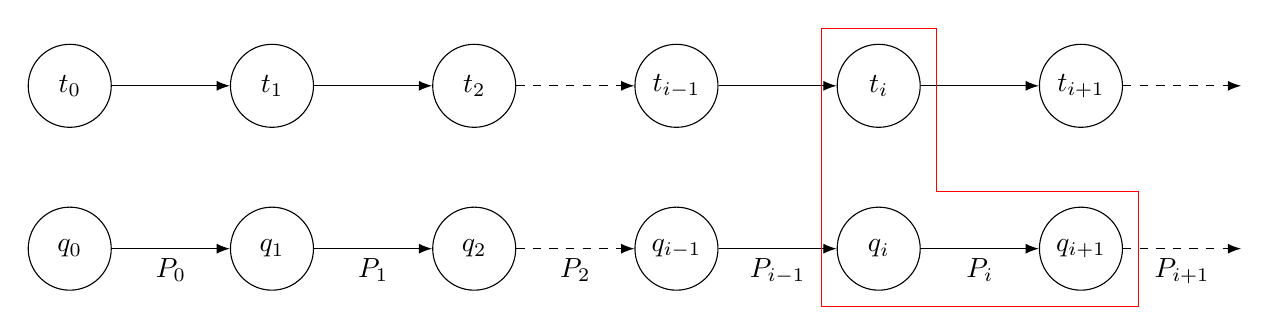
\begin{tikzpicture}[
    node distance=1cm and 1.5cm,
    state/.style={circle,draw,minimum width=3em}
    ]
    \node[state] (t0) { $t_0$ };
    \node[state] (t1) [right = of t0] { $t_1$ };
    \node[state] (t2) [right = of t1] { $t_2$ };
    \node[state] (tim1) [right = of t2] { $t_{i-1}$};
    \node[state] (ti) [right = of tim1] { $t_i$};
    \node[state] (tip1) [right = of ti] { $t_{i+1}$};
    \node (tinf) [right = of tip1] {};

    \node[state] (q0) [below = of t0] { $q_0$ };
    \node[state] (q1) [right = of q0] { $q_1$ };
    \node[state] (q2) [right = of q1] { $q_2$ };
    \node[state] (qim1) [right = of q2] { $q_{i-1}$};
    \node[state] (qi) [right = of qim1] { $q_i$};
    \node[state] (qip1) [right = of qi] { $q_{i+1}$};
    \node (qinf) [right = of qip1] {};

    \draw[-Latex] (t0) -- (t1);
    \draw[-Latex] (t1) -- (t2);
    \draw[-Latex, dashed] (t2) -- (tim1);
    \draw[-Latex] (tim1) -- (ti);
    \draw[-Latex] (ti) -- (tip1);
    \draw[-Latex,dashed] (tip1) -- (tinf);

    \draw[-Latex] (q0) -- (q1) node[midway,below] {$P_0$};
    \draw[-Latex] (q1) -- (q2) node[midway,below] {$P_1$};
    \draw[-Latex, dashed] (q2) -- (qim1) node[midway,below] {$P_2$};
    \draw[-Latex] (qim1) -- (qi) node[midway,below] {$P_{i-1}$};
    \draw[-Latex] (qi) -- (qip1) node[midway,below] {$P_i$};
    \draw[-Latex,dashed] (qip1) -- (qinf) node[midway,below] {$P_{i+1}$};

    \coordinate [above left=5mm of ti] (tial);
    \coordinate [above right=5mm of ti] (tiar);
    \coordinate [above right=5mm of qip1] (qip1ar);
    \coordinate [below right=5mm of qip1] (qip1br);
    \coordinate (middle) at (tiar |- qip1ar);
    \coordinate (qibl) at (tial |- qip1br);

    \draw[red] (tial) -- (tiar) -- (middle) -- (qip1ar) -- (qip1br) -- (qibl) --cycle;


  \end{tikzpicture}
    \caption{Synchronization of Paths from automata and from Program}
    \label{FigExplicationSynchro}
\end{figure}


\subsection{Safety}
In order to encode this approach in an approach by annotations and to consider
all program traces, our solution is to use a synchronization function. Such a
function associates the set of states synchronized with the
n$^{\textnormal{th}}$ state from an execution trace. It is the sufficient to
prove that at least one state is synchronized with each state of the execution to
establish the safety of the property.

\begin{definition}{Synchronization function}
\label{def-synchro}

Let
${A=\langle Q,q_0,R \rangle \in \textit{BUCHI}}$ and
${\sigma \in \textit{PATH}_{\textit{Prog}}}$.
The synchronization function ${\textit{Sync}\in\textit{BUCHI} \times
  \textit{PATH} \times \mathbb{N} \rightarrow 2^Q}$ is defined by:

\begin{itemize}
\item $\textit{Sync}(A,\sigma,0) = \{q_0\}$
\item {\color{darkgray}For each $i>0$:}

\centerline{
${\textit{Sync}(A,\sigma,i) =
 \left \{ q' \left |  \begin{array}{c}
                                        \exists \langle q,P,q' \rangle
                                        \in R \cdot \wedge\\
                                        \sigma_{i-1} \models
                                        P \wedge\\
                                        q \in
                                        \textit{Sync}A,\sigma,i-1)
                                      \end{array}
  \right . \right \}} $}
\end{itemize}
\end{definition}
% \vspace*{-5pt}

\begin{definition}{Acceptance condition}
% On dit qu'un automate de \buchi\ $\automate{A}$ \textbf{accept} un programme
% $\programtdefault$ si et seulement si, chaque trace $\sigma$ de
% $\programtdefault$ vrifie:\vspace*{3pt}

% \boiteGrise{0.54\textwidth}{
\centering
$(C_{Sync})$\hfill $\forall i \in 0..(\textit{len}(\sigma)-1) \cdot
\textit{Sync}(A,\sigma,i) \not = \emptyset$\hfill ~
% }
\end{definition}

This verification is encoded into annotations by generating the following assertions:

\begin{itemize}
  \item[Declaration] Let $\{q_0,\dots,q_n\}$ be a set of boolean variables
    associated to the states. $q_i$ is true if the system is synchronized with
    the state $i$. Initially, only $q_0$ is true.
  \item[Transitions] A set of ghost instructions has to be generated just before
    each call and return statement. These instructions have to update the set of
    states synchronized with the current state.
  \item[Synchronization] The synchronization condition can be expressed with an
    invariant verifying that at least one state is always synchronized.
\end{itemize}

\subsection{Liveness}

This part is not developed at this time, but the method consists in verifying a
global variant between each couple of acceptance states and also the inclusion
of the set of reachable states in the set of accepting states.

\section{Adding from the Theory}

The previous section described a sufficient framework. However, in
order to verify the correction with theorem provers, we need to use
more efficient modeling and to add some hypothesis in order to link
the models from C program and the automaton.

\subsection{ Automata Modeling}
  In order to link models from the program and the property, we describe the
  automaton as constants in the generated C file. This axiomatization is
  combined with a set of invariants that give some properties of the
  automaton. For instance, the non-reachability of a state $s$ can be deduced
  from the absence of transitions from an active state to $s$ such that its
  cross-condition is true. This cross-condition is then expressed in terms of
  program information. This is the link program-automata.


\subsection{Memorization of last Transitions}
  In order to memorize the last synchronization link, we keep the set of last
  crossed transitions in addition with the set of old active states.

\subsection{Use of Specifications instead of Invariant}
  Finally, the synchronization condition is not implemented as an invariant, but
  as a pre- and post-condition on each operation. This choice is more flexible if
  we can statically decide that some states cannot be synchronized with some
  operation. In the following section, our objective is to describe how to
  automate this simplification by using abstract interpretation.

\section{Abstract Interpretation}
{\bf Current Implementation : behavioral Property as Widening Operator}

  In this section we describe our method to generate the specification of each
  operation. In a first part, we deduce an over-approximation of specifications
  by using automata, and next we propagate the generated constraints in order to
  converge to a fixpoint of specifications.

\subsection{Generation of Abstract Specifications}
Initially, each operation's specification states that each state and transition
can be active before and after an operation.
We then fix a first constraint: the main operation starts in the initial
state. Next, we verify, for each operation, if its call or its return is always
forbidden in a particular transition's cross-condition. If any, the associated
transition is removed from the operation's specification. This process is done
once on each operation. Finally, this computed constraint has to be propagated.

\subsection{Static Simplification}
Starting from specified operations, each of them is analyzed by forward and
backward abstract interpretation. The abstraction consists in abstracting all
expressions. We only consider control statements and call and return
statements.

The post-condition is defined by intersecting its old value with the reachable
post-condition computed by forward propagation. Similarly, the pre-condition is
defined by intersecting its old value with the reachable pre-condition computed
by backward propagation.

If a loop is reached during this process, we compute its loop invariant in
terms of automata from its computed pre- and post-conditions.

During each pass of the program the list of use-cases of each operation is
kept. Hence, if we observe that an operation is still called from a strict
subset of its authorized input states, then we restrict its specification.

Finally, a fixpoint is computed in order to minimize the specifications.

Note that during this process, the post-conditions are described as
behaviors. Indeed, this approach allow to give a particular post-condition for
each possible pre-condition. Hence, the caller, which cannot observe the
control-flow inside a called operation, has more precise information about
current active states, since it knows each previous active states.

\section{Plugin Architecture}

\begin{figure}[ht]
\resizebox{\textwidth}{!}{
  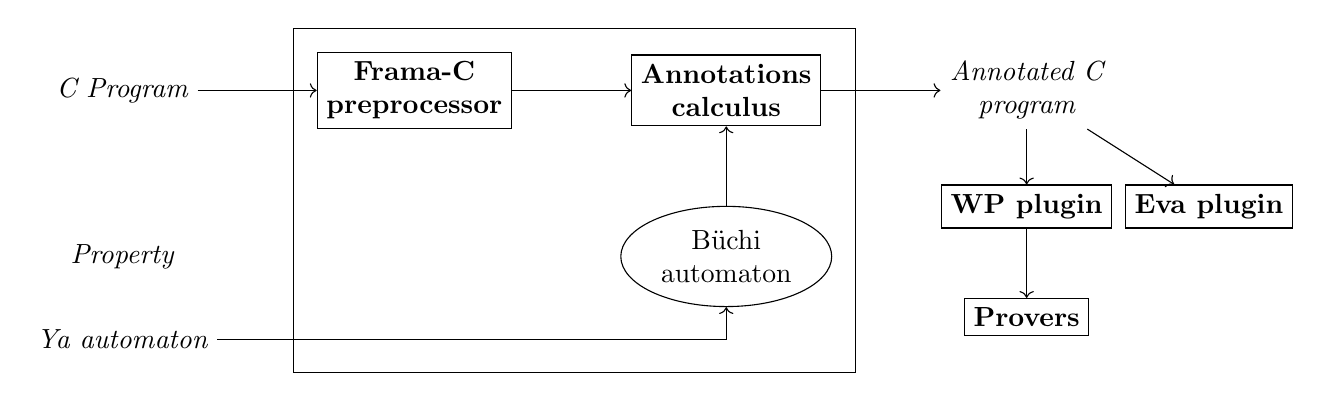
\begin{tikzpicture}
    \node (c) {\it C Program};
    \node[yshift=-6em] (prop) at (c) {\it Property};
    \node[yshift=-3em] (ya) at (prop) {\it Ya automaton};

    \node[draw,xshift=10ex,anchor=west,align=center,font=\bfseries] (fc) at (c.east) {Frama-C\\preprocessor};
    \node[draw,xshift=10ex,anchor=west,align=center,font=\bfseries] (annot) at (fc.east) {Annotations\\calculus};

    \node[ellipse,draw,yshift=-6em,align=center] (buchi) at (annot) {Büchi\\automaton};

    \node[xshift=10ex,anchor=west,align=center,font=\itshape] (prog) at (annot.east) {Annotated C\\ program};

    \node[draw,below=2em of prog] (wp) {\bf WP plugin};
    \node[draw,yshift=-4em] (provers) at (wp) {\bf Provers};
    \node[draw,below right=2em and 1ex of prog] (eva) {\bf Eva plugin};

    \node (ya2) at (ya -| buchi) {};

    \node[draw,fit=(fc) (annot) (buchi) (ya2),inner sep=3mm]{};

    \draw[->] (c) -- (fc);
    \draw[->] (fc) -- (annot);
    \draw[->] (annot) -- (prog);
    \draw[->] (prog) -- (wp);
    \draw[->] (wp) -- (provers);
    \draw[->] (prog) -- (eva);
    \draw[->] (ya) -| (buchi);
    \draw[->] (buchi) -- (annot);

  \end{tikzpicture}
}
 \caption{Plug-in Structure}
 \label{AoraiGeneralView}
\end{figure}

The plug-in is composed of three parts:
  \begin{enumerate}
    \item a front-end (translator);
    \item a computing module for specification of operations;
    \item a back-end (C generator, including annotations).
  \end{enumerate}


\section{Recent updates}
%\subsection{Frama-C+dev}

\subsection{Frama-C Iron}
\begin{itemize}
\item Remove obsolete support for LTL and Promela input language
\end{itemize}
\subsection{Frama-C Vanadium}
\begin{itemize}
\item Documentation for options \texttt{-aorai-no-generate-annotations}
and \texttt{-aorai-smoke-tests}
\item Documentation for option \texttt{-aorai-instrumentation-history}
and built-in \texttt{Frama\_C\_show\_aorai\_state}
\item Aoraï does not generate a C file by default anymore, relying on
kernel options \texttt{-print} and \texttt{-ocode} for that, like all
plug-ins. Remove corresponding ad'hoc options.
\item update syntax for YA sequence to avoid ambiguities with
 \texttt{+} and \texttt{*} repetition operators
\end{itemize}
\subsection{Frama-C Titanium}
\begin{itemize}
\item Various bug fixes
\item Introduction of YA variables
\end{itemize}
\subsection{Frama-C Aluminium}
\begin{itemize}
\item Generated functions now have a body in addition to a specification
\end{itemize}
\subsection{Frama-C Nitrogen}
\begin{itemize}
\item New translation mechanism for the automaton
\item Extended Ya guards
\end{itemize}

\subsection{Frama-C Boron}
\lstset{language=ya}
\begin{itemize}
\item A function that is used in a C program, but that is not defined
  is stubbed by Frama-C and ignored in Aorai.
\item For each function and each loop, if no state can be enabled
  before or after it (not reachable), then a warning is displayed. It
  is usually either a dead code, or a code violating the
  specification.
\item In the YA and Promela formats, it is now possible to speak about
  call parameters and returned value. \lstinline|f().a| denotes the call
  parameter \lstinline|a| of \lstinline|f| and
  \lstinline|f().return| denotes the returned value of f.
\item In the annotated C file generated, array of states are indexed
  by the name of the state (defined as an enum structure)
\end{itemize}

\subsection{Frama-C Beryllium}
\begin{itemize}
  \item YA format for properties
\end{itemize}


\chapter{Conclusion}
This manual is not always up-to-date and only gives some hints on the \aorai
plug-in. If you want more information, please send me a mail at:

\begin{center}
  nicolas.stouls@insa-lyon.fr
\end{center}

or visit the website:

\begin{center}
  \url{https://www.frama-c.com/fc-plugins/aorai.html}
\end{center}
\end{document}

Local Variables:
ispell-local-dictionary: "english"
End:
